\documentclass{article}

\usepackage{ctex}
\usepackage{tikz}
\usetikzlibrary{automata, positioning, arrows}
\usetikzlibrary{cd}

\usepackage{amsthm}
\usepackage{amsmath}
\usepackage{amssymb}
\usepackage{stmaryrd}
\usepackage{mathtools}
\usepackage{proof}

\usepackage[linesnumbered,ruled,vlined]{algorithm2e}

%\usepackage{unicode-math}
\PassOptionsToPackage{hyphens}{url}\usepackage{hyperref} %url解决过长的问题
\usepackage{hyperref} %url
\hypersetup{
    colorlinks=true,
    linkcolor=blue,
    filecolor=magenta,      
    urlcolor=cyan,
    pdftitle={Overleaf Example},
    pdfpagemode=FullScreen,
    }


\usepackage[textwidth=18cm]{geometry} % 设置页宽=18

\usepackage{blindtext}
\usepackage{bm}
\parindent=0pt
\setlength{\parindent}{2em} 
\usepackage{indentfirst}


\usepackage{xcolor}
\usepackage{titlesec}
\titleformat{\section}[block]{\color{blue}\Large\bfseries\filcenter}{}{1em}{}
\titleformat{\subsection}[hang]{\color{red}\Large\bfseries}{}{0em}{}
%\setcounter{secnumdepth}{1} %section 序号

\newtheorem{theorem}{Theorem}[section]
\newtheorem{lemma}[theorem]{Lemma}
\newtheorem{corollary}[theorem]{Corollary}
\newtheorem{proposition}[theorem]{Proposition}
\newtheorem{example}[theorem]{Example}
\newtheorem{definition}[theorem]{Definition}
\newtheorem{remark}[theorem]{Remark}
\newtheorem{exercise}{Exercise}[section]
\newtheorem{annotation}[theorem]{Annotation}

\newcommand\Set[2]{\{\,#1\mid#2\,\}} %集合
\newcommand\SET[2]{\Set{#1}{\text{#2}}} %

\newcommand{\redt}[1]{\textcolor{red}{#1}}
\newcommand{\bluet}[1]{\textcolor{blue}{#1}}
\newcommand{\abracket}[1]{\ensuremath{\left< #1 \right>}}

\newcommand*{\xfunc}[4]{{#2}\colon{#3}{#1}{#4}}
\newcommand*{\func}[3]{\xfunc{\to}{#1}{#2}{#3}}


\newcommand{\inl}[1]{\ensuremath{\text{inl}~#1}}
\newcommand{\inr}[1]{\ensuremath{\text{inr}~#1}}
\newcommand{\fold}[1]{\ensuremath{{fold}_{#1}}}
\newcommand{\unfold}[1]{\ensuremath{{unfold}_{#1}}}
\newcommand{\lam}[2]{\ensuremath{\lambda #1\ldotp #2}} %lamx.y
\newcommand{\pair}[1]{\ensuremath{\left\langle#1\right\rangle}}
\newcommand{\projone}[1]{\ensuremath{#1.1}}
\newcommand{\projtwo}[1]{\ensuremath{#1.2}}
\newcommand{\caseof}[3]{\ensuremath{{\textbf{case}}~#1~{\textbf{of}}~\inl{x_1}\mapsto #2\mid\inr{x_2}\mapsto #3}}
\newcommand{\Lam}[2]{\ensuremath{\Lambda #1\ldotp #2}}
\newcommand{\pack}[3]{\ensuremath{{pack}~\pair{#1,#2}~{as}~#3}}
\newcommand{\unpack}[4]{\ensuremath{{unpack}~#1~{as}~\pair{#2,#3}~{in}~#4}}
\newcommand{\assign}[2]{\ensuremath{#1~\coloneqq~#2}}
\newcommand{\singletype}[1]{\text{#1}}
\newcommand{\termtype}[2]{\ensuremath{#1:#2}}
\newcommand{\type}[3]{\ensuremath{ \left\{#1:#2\relmiddle|#3 \right\}}}
\newcommand{\matgen}[2]{\ensuremath{\mu #1\ldotp#2}} %ux.y
\newcommand{\mat}[0]{\matgen{\alpha}{\tau}} %ua.t
\newcommand{\fatgen}[2]{\ensuremath{\forall #1\ldotp#2}}
\newcommand{\fat}[0]{\fatgen{\alpha}{\tau}}
\newcommand{\eatgen}[2]{\ensuremath{\exists #1\ldotp#2}}
\newcommand{\eat}[0]{\eatgen{\alpha}{\tau}}
\newcommand{\fatgent}[2]{\ensuremath{\trgb{\forall} #1\ldotp#2}}
\newcommand{\fatt}[0]{\fatgent{\alpt}{\tat}}
\newcommand{\eatgent}[2]{\ensuremath{\trgb{\exists} #1\ldotp#2}}
\newcommand{\eatt}[0]{\eatgent{\alpt}{\tat}}

\newcommand{\fail}[0]{\mi{fail}}

\newcommand{\bnfdef}[0]{\ensuremath{\mathrel{::=}}} %::=
\newcommand{\term}[1]{\ensuremath\mathsf{#1}}
\newcommand{\true}{\term{true}}
\newcommand{\false}{\term{false}}
\newcommand{\ifelse}[3]{\ensuremath{\textbf{if}~#1~\textbf{then}~#2~\textbf{else}~#3}}
\newcommand{\newwhiledo}[2]{\ensuremath{\textbf{while}~#1~\textbf{do}~#2}}
\newcommand{\letvar}[2]{\ensuremath{\textbf{letvar}~#1~\textbf{in}~#2}}
\newcommand{\succt}[1]{\term{succ}~#1}
\newcommand{\pred}[1]{\term{pred}~#1}
\newcommand{\iszero}[1]{\term{iszero}~#1}
\newcommand{\seq}[2]{#1;#2}
\newcommand{\subtyp}[2]{#1<:#2}

\newcommand{\dbracket}[1]{\ensuremath{\left\llbracket\,\vcenter{\hbox{$#1$}}\,\right\rrbracket}}

\newcommand{\todo}[1]{\textcolor{red}{TODO: #1}\PackageWarning{TODO:}{#1!}}

%variable name
\ExplSyntaxOn 
\NewDocumentCommand{\vn}{m}
 {
   \seq_set_split:Nnn \l_tmpa_seq { ~ } { #1 }
   \int_compare:nTF { \seq_count:N \l_tmpa_seq > 1 }
    {
     \seq_set_map:NNn \l_tmpb_seq \l_tmpa_seq { \exp_not:N \mathit { ##1 } }
     (\seq_use:Nn \l_tmpb_seq { \  })
    }
    { \mathop{}\!\mathit{#1} }
 }
\ExplSyntaxOff

\begin{document}
\title{关于Maple Algebra的这一路}
\author{枫聆 (maplegra)}
\maketitle
\tableofcontents
\newpage

\section{Language}

\subsection{language equation and Arden's Rule}

\begin{theorem}
\rm The set $A^* \cdot B$ is the smallest language that is a solution for $X$ in the linear equation 
\[
	X = A \cdot X + B
\]
where $X, A, B$ are sets of string and $+$ stands for union of languages. Moreover, If the set $A$ does not contain the empty word, then the solution is unique.
\end{theorem}

\begin{annotation}
\rm \bluet{Arden's rule can be used to help convert some finite automatons to regular expressions}.
\end{annotation}

\newpage
\section{Equivalence of Program}

\subsection{Graph Ismorphism}

\subsection{Accepted Language Equivalentce}

\begin{annotation}
\rm \cite{CCS} Chapter 1.
\end{annotation}

\subsection{Bisimulation and Observation Equivalence}

\begin{definition}
\rm A labelled transition system (LTS) is a tuple $(S, \Lambda, \to)$ where $S$ is set of states, $\Lambda$ is set of labels, and $\to$ is relation of labelled transitions (i.e., a subset of $S \times \Lambda \times S$).  A $(p,\alpha,q) \in \to$ is written as $p  \xrightarrow{\alpha} q$. 
\end{definition}

\begin{annotation}
\rm \todo{categorical semantics: $F$-coalgebra}
\end{annotation}


\begin{definition}
\rm \cite{ITLTS}Let $T=(S,\Lambda,\to)$ be a labelled transition system. The set of \redt{traces} $\vn{Tr}(s)$, for $s \in S$ is the minimal set satisfying
\begin{itemize}
	\item $\varepsilon \in \vn{Tr}(s)$.
	\item $\alpha~\sigma \in \vn{Tr}(s)$ if $\Set{s' \in S}{s~ \xrightarrow{\alpha}~s' ~\text{and}~\sigma \in \vn{Tr}(s')}$. 
\end{itemize}
\end{definition}

\begin{definition}
\rm Two states $p,q$ are trace equivalent iff $\vn{Tr}(p) = \vn{Tr}(q)$.
\end{definition}

\begin{definition}
\rm (\redt{Simultation}) Given two labelled transition system $(S_1, \Lambda, \to_1)$ and $(S_2, \Lambda, \to_2)$, relation $R \subseteq S_1 \times S_2$ is a simulation iff, for all $(p,q) \in R$ and $\alpha \in \lambda$ satisfies
\[
	\text{for any}~p \xrightarrow{\alpha}_1 p', ~\text{then there exists}~ q'~\text{such that}~q \xrightarrow{\alpha}_2 q'~\text{and}~(p',q') \in R 	
\]
\begin{center}
% https://tikzcd.yichuanshen.de/#N4Igdg9gJgpgziAXAbVABwnAlgFyxMJZABgBpiBdUkANwEMAbAVxiRDRAF9T1Nd9CKACzkqtRizZoA5Fx7s+eAkTIBmMfWatEIAI5ze2JYOQj11TZJ27ZnMTCgBzeEVAAzAE4QAtkjIgcCCQARgsJbRAAHUjGNAALOgMQTx8kACZqQKRVMK02aNiEkGoGOgAjGAYABUUBNg8sRzicYpAGLDAIuAh2qCSU30R-LMQMto6IqDo4OIdW2bo+xDAmBgZcqxAAJVbSiura5R0GppbMuiwGNkhO-q9B0ICgxBzx250pmbnqBaWVtY2ER2dk4QA
\begin{tikzcd}
p \arrow[rrrr, "\alpha"] \arrow[ddd, "R"', dashed] &  &  &  & p' \arrow[ddd, "R", dashed] \\
                                                   &  &  &  &                             \\
                                                   &  &  &  &                             \\
q \arrow[rrrr, "\alpha"']                          &  &  &  & q'                         
\end{tikzcd}
\end{center}
\end{definition}

\begin{definition}
\rm We say $q$ simulates $p$ if there exists a simulation $R$ includes $(p,q)$ (i.e., $(p,q) \in R$), written $p < q$.
\end{definition}

%\begin{lemma}
%\rm The simulation is reflexive and transitive. 
%\end{lemma}


\begin{definition}
\rm (\redt{Bisimultation}) Given two labelled transition system $(S_1, \Lambda, \to_1)$ and $(S_2, \Lambda, \to_2)$, relation $R \subseteq S_1 \times S_2$ is a bisimulation iff both $R$ and its converse $\overline{R}$ are simulations, for all $(p,q) \in R$ and $\alpha \in \Lambda$ satisfies
\[
	\begin{gathered}
	\text{for any}~p \xrightarrow{\alpha}_1 p', ~\text{then there exists}~ q'~\text{such that}~q \xrightarrow{\alpha}_2 q'~\text{and}~(p',q') \in R \\
	\text{for any}~q \xrightarrow{\alpha}_2 q', ~\text{then there exists}~ p'~\text{such that}~p \xrightarrow{\alpha}_1 p'~\text{and}~(p',q') \in R
	\end{gathered} 	
\]
\end{definition}

%\begin{definition}
%\rm A binary relation between state transition systems, associating systems that behave in the same way in that one system simulates the other and vice versa.
%\end{definition}

\begin{example}
\rm 一些bisimulation的例子
\begin{center}
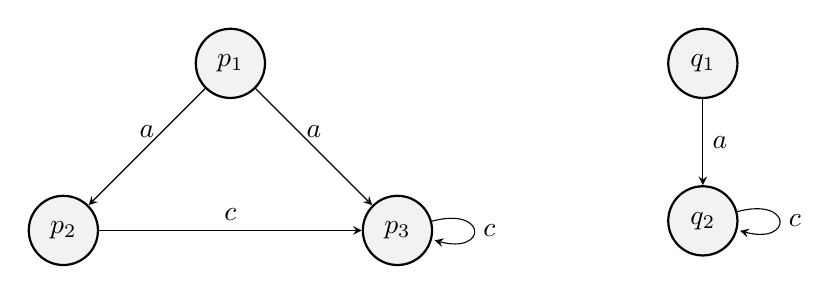
\begin{tikzpicture}
\tikzset{
->, % makes the edges directed
>=stealth, % makes the arrow heads bold
node distance=3cm, % specifies the minimum distance between two nodes. Change if necessary.
every state/.style={thick, fill=gray!10}, % sets the properties for each ’state’ node
initial text=$ $, % sets the text that appears on the start arrow
}
	\node[state] (p1) {$p_1$};
	\node[state, below left of=p1, node distance=3cm] (p2) {$p_2$};
	\node[state, below right of=p1, node distance=3cm] (p3) {$p_3$};
	\node[state, right of=p1, node distance=6cm] (q1) {$q_1$};
	\node[state, below of=q1, node distance=2cm] (q2) {$q_2$};
	
	\draw (p1) edge[above] node{$a$} (p2)
	(p1) edge[above] node{$a$} (p3)
	(p2) edge[above] node{$c$} (p3)
	(p3) edge[loop right] node{$c$} (p3)
	(q1) edge[right] node{$a$} (q2)
	(q2) edge[loop right] node{$c$} (q2);
\end{tikzpicture}
\end{center}
关于上面两个transition system的bisimultaion为$R=\{(p_1,q_1), (p_2,q_2), (p_3,q_2)\}$. 还有一个比较有点特别的例子
\begin{center}
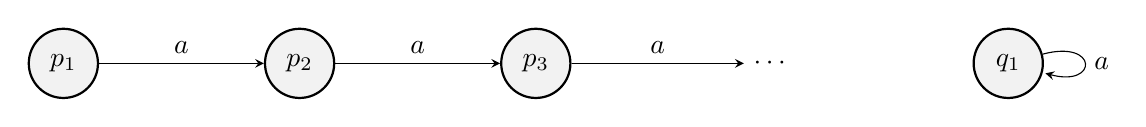
\begin{tikzpicture}
\tikzset{
->, % makes the edges directed
>=stealth, % makes the arrow heads bold
node distance=3cm, % specifies the minimum distance between two nodes. Change if necessary.
every state/.style={thick, fill=gray!10}, % sets the properties for each ’state’ node
initial text=$ $, % sets the text that appears on the start arrow
}
	\node[state] (p1) {$p_1$};
	\node[state, right of=p1, node distance=3cm] (p2) {$p_2$};
	\node[state, right of=p2, node distance=3cm] (p3) {$p_3$};
	\node[right of=p3, node distance=3cm] (p4) {$\cdots$};
	\node[state, right of=p4, node distance=3cm] (q1) {$q_1$};
	
	\draw (p1) edge[above] node{$a$} (p2)
	(p2) edge[above] node{$a$} (p3)
	(p3) edge[above] node{$a$} (p4)
	(q1) edge[loop right] node{$a$} (q1);
\end{tikzpicture}
\end{center}
如果关于上图这样bisimulation $R$存在,那么$(p_i,q_1) \in R$ for every $i$. 再看一个不是bisimulation的例子
\begin{center}
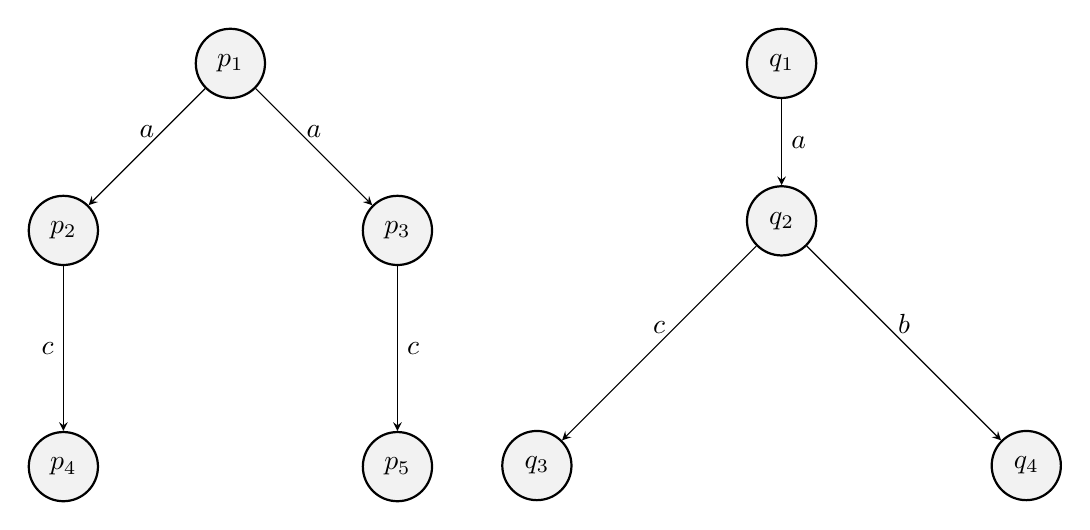
\begin{tikzpicture}
\tikzset{
->, % makes the edges directed
>=stealth, % makes the arrow heads bold
node distance=3cm, % specifies the minimum distance between two nodes. Change if necessary.
every state/.style={thick, fill=gray!10}, % sets the properties for each ’state’ node
initial text=$ $, % sets the text that appears on the start arrow
}
	\node[state] (p1) {$p_1$};
	\node[state, below left of=p1, node distance=3cm] (p2) {$p_2$};
	\node[state, below right of=p1, node distance=3cm] (p3) {$p_3$};
	\node[state, below of=p2, node distance=3cm] (p4) {$p_4$};
	\node[state, below of=p3, node distance=3cm] (p5) {$p_5$};
	\node[state, right of=p1, node distance=7cm] (q1) {$q_1$};
	\node[state, below of=q1, node distance=2cm] (q2) {$q_2$};
	\node[state, below left of=q2, node distance=4.395cm] (q3) {$q_3$};
	\node[state, below right of=q2, node distance=4.395cm] (q4) {$q_4$};
	
	\draw (p1) edge[above] node{$a$} (p2)
	(p1) edge[above] node{$a$} (p3)
	(p2) edge[left] node{$c$} (p4)
	(p3) edge[right] node{$c$} (p5)
	(q1) edge[right] node{$a$} (q2)
	(q2) edge[above] node{$c$} (q3)
	(q2) edge[above] node{$b$} (q4);
\end{tikzpicture}
\end{center}
这里不满足$(p_3, q_2) \notin R$.
\end{example}


\begin{definition}
\rm (\redt{Bisimilarity}) Given two states $p$ and $q$ in $S$, $p$ is bisimilar to $q$, written $p \sim q$,  if and only if there is a bisimulation $R$ such that $(p,q) \in R$. 
\end{definition}

\begin{definition}
\rm The bisimilarity relation $\sim$ is the union of all bisimulations.
\end{definition}

\begin{lemma}
\rm The bisimulation has some properties:
\begin{itemize}
	\item The identity relation $\vn{id}$ is a bisimulation(with two same LTS).
	\item The empty relation $\perp$ is a bisimulation.
	%\item The relation composition $R_1 \circ R_2$ of two bisimulation $R_1$ and $R_2$ is a bisimulation.
	\item (\redt{closed under union}) The $\bigcup_{i \in I} R_i$ of a family of bisimulations $(R_i)_{i \in I}$ is a bisimulation.
\end{itemize}
\end{lemma}

\begin{lemma}
\rm \cite{AITBAC} The bisimilarity relation $\sim$ is equivalence relation (i.e., reflexivity, symmetry, transitivity).
\end{lemma}

\begin{proof}
\rm 其中reflexivity, symmetry是比较显然的. Transitivity稍微麻烦一点,我们用relation composition定义新的relation$R_3 = R_1;R_2$, 此时有$(p,q) \in R_3$,因此只要证明$R_3$ is bisimulation足够了. 取任意一个$(p_1, q_1) \in R_3$,那么按照$R_3$的定义, 存在$(p_1, r_1) \in R_1$和$(r_1, q_1)$. 由$p_1 \sim r_1$那么对于任意的$p_1 \xrightarrow{\alpha} p_1'$, 存在$r_1 \xrightarrow{\alpha} r_1'$满足$(p_1',r_1') \in R_1$. 再由$r_1 \sim q_1$, 存在$q_1 \xrightarrow{\alpha} q_1'$满足$(r_1',q_1') \in R_2$. 于是按照$R_3$的定义也有$(p_1', q_1') \in R_3$. 再由$R_2$ is bisimulation, 从$(r_1,q_1) \in R_2$按照上述的思路往回证明即可,最终$R_3$ is bisimulation.
\end{proof}

\begin{definition}
\rm \cite{mLTS} An LTS is called \redt{deterministic} if for every state $p$ and action $\alpha$, there is at most one state $q$ such that $p \xrightarrow{\alpha} q$.
\end{definition}

\begin{lemma}
\rm In a deterministic LTS, two states are bisimilar if and only if they are trace equivalent,
\[
	s_1 \sim s_2 \iff \vn{Tr}(s_1)=\vn{Tr}(s_2)
\]
\end{lemma}

\begin{proof}
\rm 

先证$\Rightarrow$, 设满足$s_1 \sim s_2$($(s_1,s_2) \in R$ and $R$ is bisimultaion), 设$\sigma_{s_1} \in \vn{Tr}(s_1)$, 其中$\sigma_{s_1}$为sequence $(\alpha_i)_{i \in I}$ where $I$ is a indexed famliy. 由于$s_1 \sim s_2$, 那么对于$s_1 \xrightarrow{\alpha_1} s_1'$, 存在$s_2 \xrightarrow{\alpha_1} s_2'$, 于是$(s_1',s_2') \in R$, 根据$\sigma$长度做induction可以证明$\sigma_{s_1} \in \vn{Tr}(q)$. 再反过来证明$\sigma_{s_2} \in \vn{Tr}(s_2)$也同样有$\sigma_{s_2} \in \vn{Tr}(s_1)$. 最终$\vn{Tr}(s_1)=\vn{Tr}(s_2)$.

对于$\Leftarrow$, 我们可以用$\vn{Tr}(s_1) = \vn{Tr}(s_2)$构造一个bisimulation, 定义relation $R$为
\[
 	\vn{Tr}(s_1) = \vn{Tr}(s_2) \iff (s_1,s_2) \in R.
\]
只要能证明$R$ bisimulation即可. 首先我们来说明在deterministic限制下一个比较好性质: 若$\vn{Tr}(s_1) = \vn{Tr}(s_2)$且当$s_1 \xrightarrow{\alpha} s_1', s_2 \xrightarrow{\alpha} s_2'$, 那么$\vn{Tr}(s_1') = \vn{Tr}(s_2')$. 这样对于任意地$(s_1,s_2) \in R$, 它们accept相同action对应的transition $(s_1', s_2') \in R$. 因此$s_1 \sim s_2$. 
\end{proof}


\begin{definition}
\rm (\redt{Weak Bisimultation}) Given two labelled transition system $(S_1, \Lambda, \to_1)$ and $(S_2, \Lambda, \to_2)$, relation $R \subseteq S_1 \times S_2$ is a bisimulation iff both $R$ and its converse $\overline{R}$ are simulations, for all $(p,q) \in R$ and $\alpha \in \Lambda \cup \{\tau\}$ satisfies
\[
	\begin{gathered}
	\text{for any}~p \xrightarrow{\alpha}_1 p', ~\text{then there exists}~ q'~\text{such that}~q \xrightarrow{\tau*~\alpha~\tau*}_2^* q'~\text{and}~(p',q') \in R \\
	\text{for any}~q \xrightarrow{\alpha}_2 q', ~\text{then there exists}~ p'~\text{such that}~p \xrightarrow{\tau*~\alpha~\tau*}_1^* p'~\text{and}~(p',q') \in R
	\end{gathered} 	
\]
where $\xrightarrow{}^*$ is multi-transition.
\end{definition}


\begin{annotation}
\rm \bluet{对于LTS的一些想法}:
\begin{itemize}
	\item 如果你想用transition system来做reasoning可以考虑把它和Kripke frame联系起来,同时要构造一些modality来设计方便做reasoning的calculus.
	\item (\emph{bisimulation proof method}) 对于两个特别的states来说,我们应该如何找到这样bisimulation来满足$(p,q) \in R$?
	\item 对于两个特别的LTS来说,我们怎样以bisimulation思考它们是否equivalent? bisimulation的最初定义应该叫做strong bisimulation, 它建立的是一种strong equivalence, 而weak bisimulation建立是一种observation equivalence.
\end{itemize}
\end{annotation}

\begin{annotation}
\rm  \todo{CCS(calculus of communicating systems)\cite{CCS} and mCRL2 \cite{mLTS}}.
\end{annotation}

\newpage
\begin{thebibliography}{9}
\bibitem{ITLTS}
Introduction to labelled transition systems. \newline\url{http://wiki.di.uminho.pt/twiki/pub/Education/MFES1617/AC/AC1617-2-LTS.pdf}

\bibitem{AITBAC}
An Introduction to Bisimulation and Coinduction. \newline\url{https://homes.cs.washington.edu/~djg/msr_russia2012/sangiorgi.pdf}

\bibitem{mLTS}
Labelled transition systems. \newline\url{https://www.mcrl2.org/web/user_manual/articles/lts.html}


\bibitem{CCS}
A Calculus of Communicating Systems. Robin Milner. 

\end{thebibliography}
\end{document}